%% wrap_S4.tex — Supplementary Material S4: Numerical Checks
%% Compile: xelatex wrap_S4.tex (from supplementary/src/), then bibtex, then xelatex x2
%% Output:  supplementary/S4_numerical_checks.pdf

\documentclass[a4paper,12pt]{article}
\usepackage[utf8]{inputenc}
\usepackage[T1]{fontenc}
\usepackage{amsmath,amssymb}
\usepackage{booktabs}
\usepackage{graphicx}
\usepackage{microtype}
\usepackage[numbers,sort&compress]{natbib}
\usepackage[hidelinks]{hyperref}
\usepackage{placeins}
\usepackage{geometry}
\geometry{margin=2.5cm}

%% No-op revision macros from the main article
\DeclareRobustCommand{\warn}[1]{}
\providecommand{\added}[1]{#1}
\providecommand{\changed}[2]{#2}
\providecommand{\deleted}[1]{}

%% Cross-reference to the accumulation-bound equation in the main text.
%% \eqref{eq:accumulate} appears in S4.tex; it refers to Eq. (2) of the paper.
\makeatletter
\global\@namedef{r@eq:accumulate}{{2}{2}}
\makeatother

\title{%
  Supplementary Material S4: Numerical Checks of Formal Results in Their Own Models\\[4pt]
  {\large\normalfont
    Recursive Training on Model-Generated Data: A Critical Integrative Review\\
    of Failure Regimes, Adversarial Interactions and Governance}\\[2pt]
  {\small\normalfont
    Azancort Neto, J.L.; Ferreira de Carvalho, A.C.P.L.; Franc\^es, C.R.L.\\
    \textit{Computer Science Review} (2026), COSREV-D-26-01510}
}
\author{}
\date{}

\begin{document}
\maketitle
\thispagestyle{empty}
\tableofcontents
\clearpage

%% S4.tex — Numerical check of Results 1, 2 and 5
%% Included in the submission package; not compiled into the main PDF.
%% All numbers in this file come from sim/s4a_results.json
%% (seed 20261029, generated at the gate-v3 commit listed in MANIFEST.txt).

\section*{S4. Numerical check of formal results in their own models}

\paragraph{Purpose and scope.}
This supplement checks numerically, in the models in which they are proved, formal
results summarised in Section~2.1 and Table~2 of the main text. It does not test
whether these results transfer to transformer language models, which remains an open
question (Section~7.5, priority~1). All runs use seed 20261029; the scripts and
their raw output are available at the repository listed under Code Availability.
Run time: 4.8~s on a single CPU core.

\paragraph{S4.1~Linear regression: replacement, accumulation and a fixed budget
(Results~1--2).}
\emph{Setting.} Ordinary least squares with $d=10$, $N=50$ samples per
generation, noise variance $\sigma^2=1$, a fixed true parameter $\theta^\ast$ and
isotropic Gaussian inputs drawn afresh at each generation\footnote{Whether
Gerstgrasser et al.\ use fixed or fresh inputs is verified against their theorem
statement; see main text, \warn{3}.}; at generation $g\ge1$ labels are produced
by the previous model of the same regime plus $\mathcal N(0,\sigma^2)$ noise;
generations $0$--$20$; $R=300$ replicates.
\emph{Regimes.} \textit{Replace}: fit on the new batch only.
\textit{Accumulate}: fit on the real data and all synthetic batches.
\textit{Accumulate-subsample}: fit on a uniform random subset of $2N$ points from
the accumulated pool (a stand-in for a fixed training budget).
\emph{Outcome}: $E_g = \mathbb{E}\lVert\hat\theta_g-\theta^\ast\rVert^2$,
normalised by $E_0 = \sigma^2 d/(N{-}d{-}1) = 0.256$.

\emph{Results (Table~S4.1a, Fig.~S4.1a).}
Under replacement the error follows $E_0(g+1)$ closely (maximum relative
deviation $5.4\%$ at $g=1$, within the 95\% CI).
Under accumulation it stays below $E_0\sum_{i=1}^{g+1}i^{-2}$ at every generation
and below $E_0\pi^2/6 = 1.64\,E_0$ ($1.58\pm0.11\,E_0$ at $g=20$).
Under a fixed budget it exceeds $E_0\pi^2/6$ at $g=4$ and reaches
$2.05\pm0.12\,E_0$ at $g=20$, still rising slowly: the bound of Result~2 requires
every fit to use all retained data, not a fixed-size subsample.

\paragraph{S4.2~Gaussian mean estimation with a growing synthetic sample
(Result~5).}
\emph{Setting.} $\theta^\ast=0$, $\sigma=1$; initial real sample $n=20$; at
iteration $t\ge2$ the estimate is the mean of $n_t=\lceil c_{t-1}\,n\rceil$ samples
drawn from $\mathcal N(\hat\theta_{t-1},1)$; schedules $c_k=1$, $c_k=k$ and
$c_k=k^{1.5}$; $T=200$; $R=20{,}000$ replicates.
In this model $n\,\mathbb{E}[(\hat\theta_T-\theta^\ast)^2]
= 1 + \sum_{t=2}^{T} n/n_t$ exactly.

\emph{Results (Table~S4.1b, Fig.~S4.1b).}
With a constant schedule the error grows linearly; with a linear schedule it grows
as $O(\log T)$ and is therefore unbounded; with $c_k=k^{1.5}$ it converges to a
finite limit (observed $3.45$ at $T=200$, below $1+\zeta(1.5)\approx3.61$).
The probability of improvement
$P(T)=\Pr(|\hat\theta_T-\theta^\ast|<|\hat\theta_1-\theta^\ast|)$ is below
$\tfrac12$ for every schedule and $T$: at $T=2$ it is $0.355\pm0.007$, against the
exact value $\tfrac12 - \pi^{-1}\arcsin(5^{-1/2}) \approx 0.352$.
Under $c_k=k^{1.5}$ the error is bounded while $P(200) = 0.288\pm0.006$: a
probability below $\tfrac12$ is compatible with bounded error
(Section~2.1, Result~5, ``probability of improvement'' remark).

\paragraph{What the supplement does not show.}
These simulations reproduce theorems in the models in which they are proved.
They do not test whether Results~1, 2 or~5 hold for transformer language models,
which is priority~(1) of Section~7.5 of the main text.

\begin{table}[h]
\caption{Numerical check of Results~1, 2 and~5. Means shown with 95\% confidence
intervals where $R\ge100$. All numbers from \texttt{sim/s4a\_results.json},
seed 20261029.}
\label{tab:S4-1}
\small
\begin{tabular}{lrrr}
\toprule
\multicolumn{4}{l}{\emph{(a) Linear regression, $E_g/E_0$; $d=10$, $N=50$, $R=300$}} \\
$g$ & Replace (vs $g+1$) & Accumulate (vs $\sum i^{-2}$) & Accsub ($2N$ budget) \\
\midrule
1  & $2.11\pm0.12$ \ (2)   & $1.29\pm0.09$ \ (1.25) & $1.28\pm0.09$ \\
5  & $5.94\pm0.30$ \ (6)   & $1.48\pm0.10$ \ (1.49) & $1.79\pm0.10$ \\
20 & $20.70\pm1.05$ (21)   & $1.58\pm0.11$ \ (1.60) & $2.05\pm0.12$ \\
\midrule
\multicolumn{4}{l}{\emph{(b) Gaussian mean, $n\,E_T$ (sim / exact) and $P(T)$; $n=20$, $R=20{,}000$}} \\
Schedule & $T=2$ (/ exact) & $T=200$ (/ exact) & $P(200)\pm95\%$ \\
\midrule
$c_k=1$         & $1.99$ / $2.00$ & $200.0$ / $200.0$ & $0.044\pm0.003$ \\
$c_k=k$         & $2.03$ / $2.00$ & $7.01$  / $6.87$  & $0.220\pm0.006$ \\
$c_k=k^{1.5}$   & $1.97$ / $2.00$ & $3.45$  / $3.47$  & $0.288\pm0.006$ \\
\bottomrule
\end{tabular}
\end{table}

\paragraph{Figure S4.1.}
(a)~Normalised excess risk in linear regression under replacement, accumulation and
accumulate-subsample ($2N$ budget); dashed: $g+1$ (Result~1); dotted:
$\sum_{i\leq g+1}i^{-2}$ (Result~2); grey horizontal: $\pi^2/6$; bands: 95\% CI
over 300 replicates. (b)~Normalised error of recursive Gaussian mean estimation
under three synthetic-sample schedules (log--log); dashed: exact value; dotted:
$1+\zeta(1.5)$.

% ── S4.3–S4.5 (added in item 8b) ──────────────────────────────────────────────
%
% Numbers from sim/s4b_results.json, seed 20261029, runtime 3.6 s.

\paragraph{S4.3~Linear regression with a fixed input design (Results~1--2).}
\emph{Setting.} As in S4.1 but one input matrix $X\in\mathbb{R}^{N\times d}$ per
replicate is reused at every generation; $R=300$.
\emph{Results} (Table~S4.2a, Fig.~S4.2c). Replacement follows $E_0(g+1)$ closely
($2.04\pm0.12$ at $g=1$, $20.23\pm1.07$ at $g=20$). Accumulation at $g=20$ is
$1.54\pm0.08\,E_0$; the theory value $\sum_{i=1}^{21}i^{-2}=1.598$ lies within the
95\% confidence interval $[1.46, 1.62]$, so the result is consistent with
Theorem~2 of~\cite{gerstgrasser2024colm}\warn{3}. With fresh inputs (S4.1)
accumulation remains below this value: the bound of~\eqref{eq:accumulate} requires
a fixed input design.

\paragraph{S4.4~Discrete distribution with a fixed sample size (Result~4).}
\emph{Setting.} $K=50$ outputs with $p_k\propto k^{-1.2}$; $N=500$ samples per
generation; $G=100$ generations; $R=300$. \emph{Replace}: each generation is the
empirical distribution of $N$ samples drawn from the previous one. \emph{Accumulate}:
the original samples are kept and $N$ new samples are added per generation.
\emph{Results} (Table~S4.2b, Fig.~S4.2a). Under replacement support falls from
$46.0$ to $6.8$ outputs and the total-variation distance to $p$ rises from $0.10$
to $0.58$. An output's survival time grows with its expected initial count
$m_k = Np_k$ (correlation $0.97$ across outputs with census rate below $20\%$) and
exceeds $m_k$ in $74.9\%$ of output--replicate pairs, consistent with the lower
bound of~\cite{suresh2025rate}; the ratio of survival time to $m_k$ ranges from
$7.0$ to $4.1$ (Table~S4.2b), so the simulation does not show strict
proportionality.
Under accumulation the support cannot shrink, because the original samples are
retained; the total-variation distance to $p$ rises from $0.10$ to $0.12$ and
then stabilises, consistent with bounded drift.

\paragraph{S4.5~Temperature-filtered sampling under accumulation (Result~6).}
\emph{Setting.} Exact-tracking limit of~\cite{marchi2024heatdeath} ($\delta=0$):
$K=20$ outputs, $200$ initial samples from $p_k\propto k^{-1.1}$, then $2{,}000$
steps of $b=10$ samples drawn from $q^{1/T_{\mathrm s}}/\sum_k q_k^{1/T_{\mathrm s}}$;
$T_{\mathrm s}\in\{0.8,1.0,1.25\}$; $R=200$.
\emph{Results} (Table~S4.2c, Fig.~S4.2b). With $T_{\mathrm s}=1.0$ the distribution
drifts and stabilises (total-variation distance between steps $1{,}000$ and
$2{,}000$: $0.010$; normalised entropy $0.79\to0.78$), consistent with bounded drift
(Theorem~1 of~\cite{marchi2024heatdeath}). With $T_{\mathrm s}=1.25$ entropy rises
towards $1$ ($0.79\to0.95$), i.e.\ towards the uniform distribution. With
$T_{\mathrm s}=0.8$ mass concentrates (entropy $0.79\to0.24$; largest output share
$0.31\to0.82$); no output reaches zero in finite time because counts only increase,
which corresponds to approach towards the simplex boundary. These three regimes match
those of Theorems~1--3 of~\cite{marchi2024heatdeath}.

\begin{table}[h]
\caption{Numerical check of Results~1--2 (fixed design), 4 and~6. All numbers
from \texttt{sim/s4b\_results.json}, seed 20261029.}
\label{tab:S4-2}
\small
\begin{tabular}{lrrrr}
\toprule
\multicolumn{5}{l}{\emph{(a) Fixed-design regression, $E_g/E_0$ (95\% CI);
  $d=10$, $N=50$, $R=300$}} \\
$g$ & Replace & $g+1$ & Accumulate & $\sum_{i\leq g+1}i^{-2}$ \\
\midrule
1  & $2.04\pm0.12$ & 2  & $1.23\pm0.06$ & 1.250 \\
5  & $5.85\pm0.31$ & 6  & $1.45\pm0.08$ & 1.491 \\
20 & $20.23\pm1.07$ & 21 & $1.54\pm0.08$ & 1.598 \\
\midrule
\multicolumn{5}{l}{\emph{(b) Discrete distribution: support size / TV to $p$;
  $K=50$, $N=500$, $R=300$}} \\
$g$ & \multicolumn{2}{c}{Replace} & \multicolumn{2}{c}{Accumulate ($T_s=1$)} \\
\midrule
0   & \multicolumn{2}{c}{46.0 / 0.10} & \multicolumn{2}{c}{46.0 / 0.10} \\
10  & \multicolumn{2}{c}{24.1 / 0.29} & \multicolumn{2}{c}{46.0 / 0.12} \\
100 & \multicolumn{2}{c}{\hphantom{2}6.8 / 0.58} &
    \multicolumn{2}{c}{46.0 / 0.12} \\
\midrule
\multicolumn{5}{l}{\emph{(c) Temperature-filtered accumulation after
  $20{,}000$ additional samples; $K=20$, $R=200$}} \\
$T_{\mathrm s}$ & $H(q)/\log K$ & TV to $q_0$ & Largest share
  & TV steps 1k--2k \\
\midrule
0.8  & 0.24 & 0.52 & 0.82 & 0.058 \\
1.0  & 0.78 & 0.10 & 0.32 & 0.010 \\
1.25 & 0.95 & 0.28 & 0.13 & 0.029 \\
\bottomrule
\end{tabular}
\end{table}

\paragraph{Figure S4.2.}
(a)~Support size under replacement and accumulation ($K=50$, $N=500$; under
accumulation support is fixed at its initial value by construction). Bands: 10--90\%
quantiles over replicates.
(b)~Normalised entropy $H(q)/\log K$ under temperature-filtered accumulation;
dashed: uniform ($H=1$); dotted: $H(p)$. Bands: 10--90\% quantiles.
(c)~Fixed-design regression; dashed: $g+1$ (Result~1); dotted:
$\sum_{i\leq g+1}i^{-2}$ (Result~2); bands: 95\% CI of the mean.


%% ---- Figures (the S4.tex paragraphs describe these; images included here) ----
\FloatBarrier
\clearpage
\section*{Figures}

\begin{figure}[htbp]
\centering
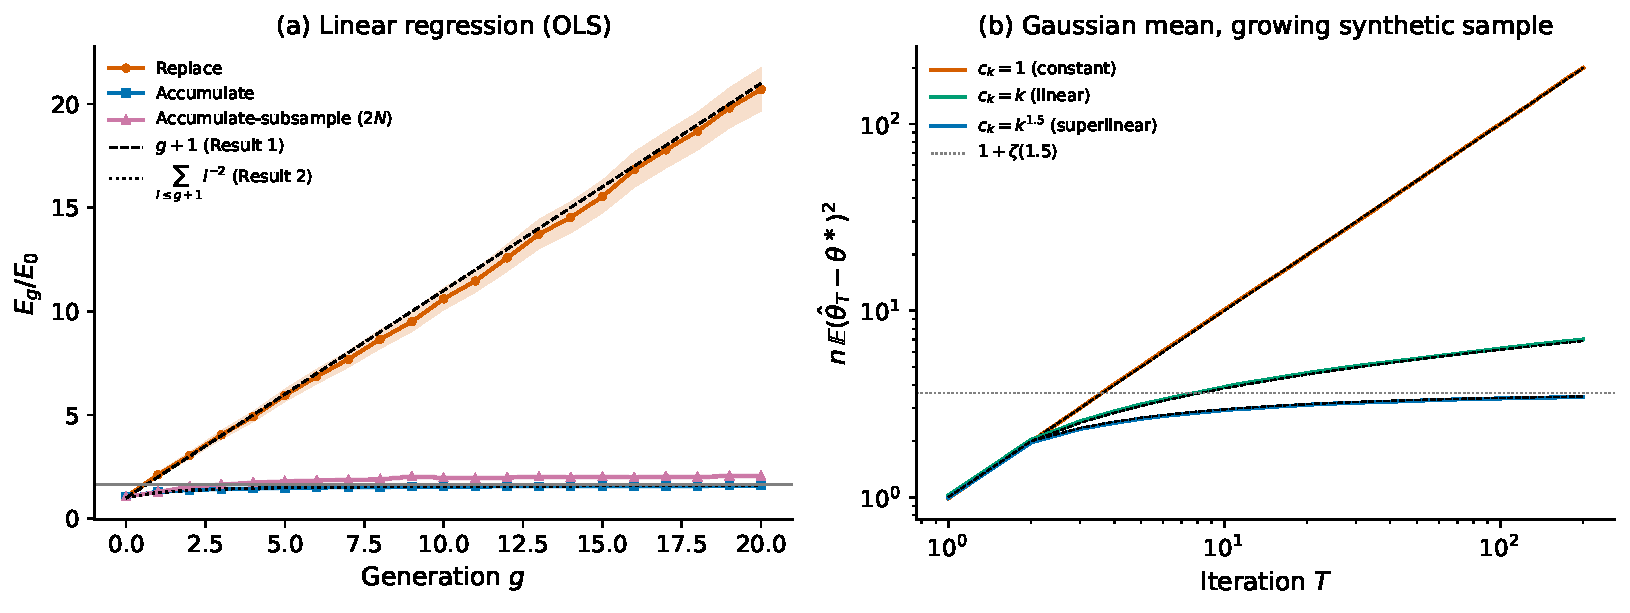
\includegraphics[width=\textwidth]{../../sim/figS4_1}
\caption{\textbf{Figure S4.1.}
(a)~Normalised excess risk in linear regression under replacement, accumulation and
accumulate-subsample ($2N$ budget); dashed: $g+1$ (Result~1); dotted:
$\sum_{i\leq g+1}i^{-2}$ (Result~2); grey horizontal: $\pi^2/6$; bands: 95\% CI
over 300 replicates.
(b)~Normalised error of recursive Gaussian mean estimation under three
synthetic-sample schedules (log--log); dashed: exact value; dotted: $1+\zeta(1.5)$.
All numbers from \texttt{sim/s4a\_results.json}, seed 20261029.}
\label{fig:S4-1}
\end{figure}

\begin{figure}[htbp]
\centering
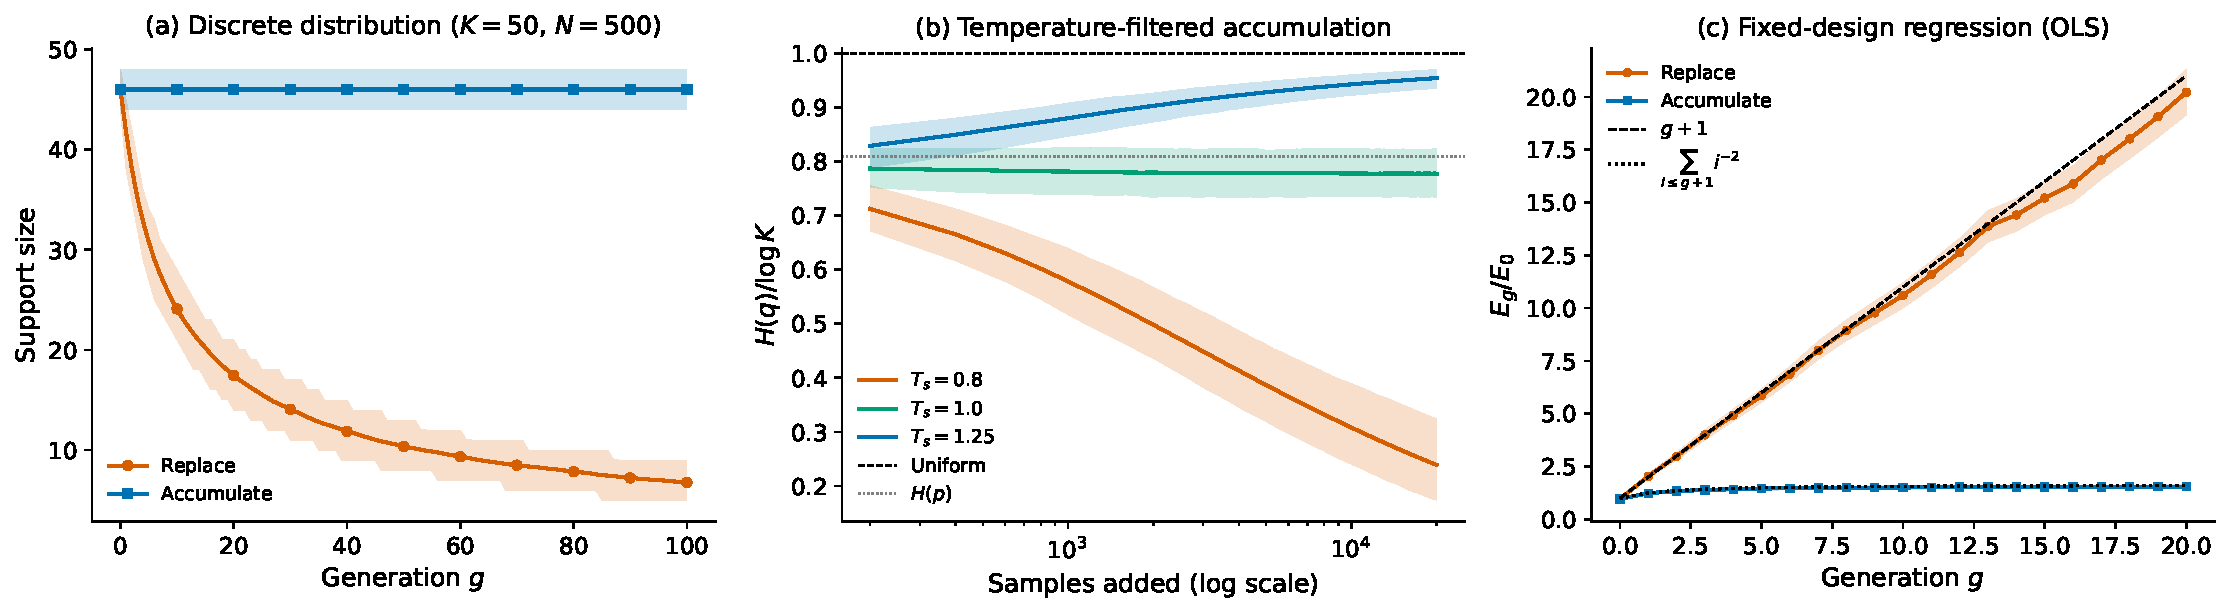
\includegraphics[width=\textwidth]{../../sim/figS4_2}
\caption{\textbf{Figure S4.2.}
(a)~Support size under replacement and accumulation ($K=50$, $N=500$; under
accumulation support is fixed by construction). Bands: 10--90\% quantiles.
(b)~Normalised entropy $H(q)/\log K$ under temperature-filtered accumulation;
dashed: uniform ($H=1$); dotted: $H(p)$. Bands: 10--90\% quantiles.
(c)~Fixed-design regression; dashed: $g+1$ (Result~1); dotted:
$\sum_{i\leq g+1}i^{-2}$ (Result~2); bands: 95\% CI.
All numbers from \texttt{sim/s4b\_results.json}, seed 20261029.}
\label{fig:S4-2}
\end{figure}

\FloatBarrier
\bibliographystyle{plainnat}
\bibliography{sn-bibliography}

\end{document}
